\documentclass[tikz]{standalone}

\usepackage[T1]{fontenc}
\usepackage[english]{babel}

\usepackage{tikz}

\begin{document}

	\begin{tikzpicture}
		\node[visible on=<1>] (image) {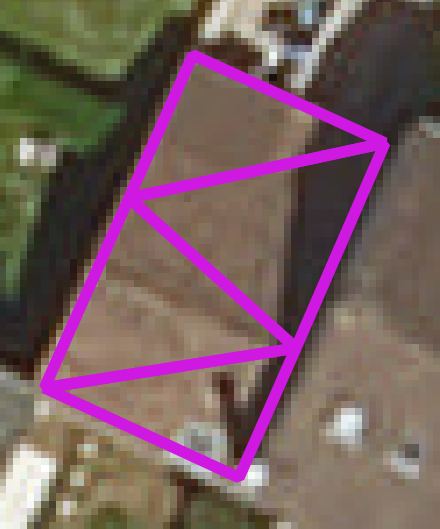
\includegraphics[width=1.5cm, angle=270]{images/introduction/graphical_abstract/orthoprojection}};
		\path (image.south) node[anchor=north, visible on=<1>, text width=1.5cm] (image_legend) {\scriptsize Nadir projection on orthoimage.};

		\path (image) node[visible on=<2>] (pixel_segment) {\includestandalone[width=1.5cm]{figures/features/radiometric_features}};

		\path (image) node[visible on=<3->] (segment_hist) {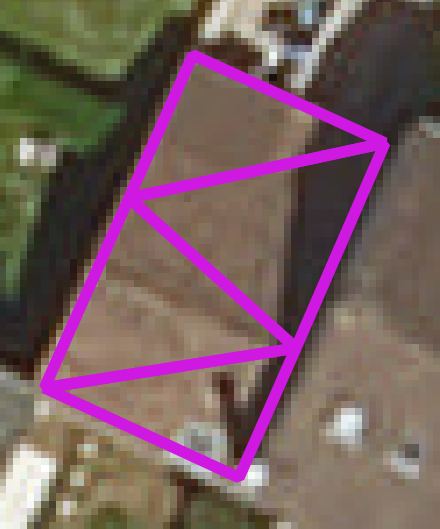
\includegraphics[width=1.5cm, angle=270]{images/introduction/graphical_abstract/orthoprojection}};

		% \path (image) + (1, 0) node[visible on =<3>] (segment_hist_1) {
		% 	\resizebox{.5cm}{.5cm}{
		% 		\begin{tikzpicture}background rectangle/.style={fill=white}, show background rectangle
		% 			\begin{axis}[
		% 				area style,
		% 				ymin=0,
		% 				ytick=\empty,
		% 				xtick=\empty,
		% 				visible on=<3>
		% 			]
		% 				\addplot+[ybar interval,mark=no] plot coordinates {
		% 					(-8, 3623)
		% 					(-7, 546)
		% 					(-6, 159)
		% 					(-5, 182)
		% 					(-4, 70)
		% 				};
		% 			\end{axis}
		% 		\end{tikzpicture}
		% 	}
		% };
	\end{tikzpicture}
\end{document}
